% This is samplepaper.tex, a sample chapter demonstrating the
% LLNCS macro package for Springer Computer Science proceedings;
% Version 2.25 of 2026/09/03
%
\documentclass[runningheads]{llncs}
%
\usepackage[T1]{fontenc}
% T1 fonts will be used to generate the final print and online PDFs,
% so please use T1 fonts in your manuscript whenever possible.
% Other font encondings may result in incorrect characters.
%

\usepackage{newtxtext}       % 
\usepackage[varvw]{newtxmath}       % selects Times Roman as basic font


\usepackage{graphicx}
\usepackage{float}

\graphicspath{ {img/}{figuras/} }
\raggedbottom  % sin esto LLNCS estira el texto para rellenar la página cuando una figura [H] no cabe


\begin{document}
\title{Práctica 2: Aprendizaje Federado}

\author{Alicia Losada Sánchez \and
Carlos Orejuela Lluncor \and
Hugo Varela Sánchez}


\institute{Aprendizaje Automático a Gran Escala, Universidade da Coruña}

\maketitle

\begin{abstract}
Desarrollo de un sistema federado simulado en un solo ordenador empleando el conjunto
de datos de \textit{Fashion-MNIST}. Se gestionaron tareas, tales como el reparto de datos 
entre los clientes utilizando variantes como IID, Dirichlet y Dirichlet Shards, el entrenamiento 
de los modelos locales (MLP y CNN) en los clientes y la recepción de sus actualizaciones en el 
servidor para realizar la agregación mediante algoritmos como FedAVG y SCAFFOLD. También se 
registró el coste de las comunicaciones implicadas dentro de este proceso. El objetivo principal 
junto con estas implementaciones es realizar diferentes experimentos que permitan evaluar el 
impacto de la heterogeneidad de los datos en un sistema federado mediante el registro de resultados 
y gráficas, así como la variación de los hiperparámetros tanto del lado del cliente como el del servidor.

\keywords{Particionado, Modelos locales, Agregación de resultados}
\end{abstract}



\section{Repartición de datos}

\subsection{IID}

\subsection{Dirichlet} 

\subsection{Dirchlet Shards}

\section{Modelos implementados}

\subsection{MLP}
Se implementó el perceptrón multicapa de las diapositivas como una subclase de \texttt{nn.Sequential}. La entrada
de tamaño $(1, 28, 28)$ se aplana con \texttt{nn.Flatten} y atraviesa dos capas ocultas de 200 neuronas con activación
ReLU, seguidas de una capa de salida de 10 neuronas:
\[
784 \rightarrow 200 \rightarrow 200 \rightarrow 10
\]
La última capa devuelve directamente los \textit{logits}, sin aplicar \textit{softmax}, ya que la función de pérdida
de PyTorch (\texttt{cross\_entropy}) la incorpora internamente. El número de neuronas ocultas se lee del parámetro
\texttt{hidden} de la configuración, y con el valor por defecto el modelo tiene 199.210 parámetros.

\subsection{CNN}
Como punto de partida se tomó la red convolucional del artículo original de FedAvg~\cite{mcmahan}, formada por dos
convoluciones $5 \times 5$ de 32 y 64 canales, cada una seguida de ReLU y \textit{max pooling} $2 \times 2$, una
capa densa de 512 neuronas y la capa de salida. Esta red tiene 1.663.370 parámetros, de los que el 96.6\,\%
pertenecen a la capa densa, por lo que se eliminó dicha capa para cumplir con el límite de 100.000 parámetros,
manteniendo las convoluciones tal y como aparecen en el artículo. Además, se tomaron las siguientes decisiones de
diseño, orientadas al entrenamiento federado con datos no-IID:

\begin{itemize}
    \item \textbf{Sin BatchNorm}: esta capa normaliza con la media y la varianza de cada mini-lote, que con datos
    no-IID dependen de la distribución local del cliente y no se parecen a las del conjunto global, lo que degrada
    FedAvg~\cite{hsieh}.
    \item \textbf{Red ancha y poco profunda}: con datos no-IID, aumentar la profundidad empeora los resultados,
    mientras que aumentar la anchura los mejora~\cite{divergencia}. Por ello, los parámetros se emplean en canales
    y no en capas.
    \item \textbf{Aplanado y capa lineal}: en lugar de \textit{global average pooling}, que con datos no-IID deja
    una entrada demasiado pequeña al clasificador y empeora el resultado~\cite{divergencia}.
    \item \textbf{Sin \textit{dropout} ni \textit{weight decay}}, y con los mismos hiperparámetros de entrenamiento
    que el MLP, de modo que la comparación entre ambos modelos solo dependa de la arquitectura.
\end{itemize}

A partir de este diseño se consideraron tres variantes:

\begin{itemize}
    \item \textbf{CNN sin GroupNorm} (83.466 parámetros): la red descrita, que fue la variante inicial.
    \item \textbf{CNN $3 \times 3$ sin GroupNorm} (50.186 parámetros): la misma red con filtros $3 \times 3$, con
    menor campo receptivo y menor coste.
    \item \textbf{CNN con GroupNorm} (83.658 parámetros): la variante inicial con GroupNorm~\cite{groupnorm} tras
    cada convolución, con 8 grupos. A diferencia de BatchNorm, normaliza cada ejemplo por separado, sin emplear
    estadísticas del mini-lote, por lo que no presenta el problema anterior y recupera gran parte de la pérdida
    que sufren los modelos normalizados con datos no-IID~\cite{hsieh}.
\end{itemize}

Para la elección de la mejor variante de CNN se tomó como criterio la \textit{accuracy} final sobre el conjunto de
test, calculada como la media de las 5 últimas rondas de cada ejecución y promediada entre 3 semillas, con IID y
Dirichlet $\alpha=0.1$. Se mantendría la variante inicial salvo que otra la superase en $\alpha=0.1$ por más de una
desviación típica:

\begin{table}[H]
    \centering
    \caption{\textit{Accuracy} final de las variantes de CNN (media $\pm$ desviación típica entre 3 semillas)}
    \label{tab:cnn_variantes}
    \setlength{\tabcolsep}{5pt}
    \begin{tabular}{lccc}
        \hline
        Variante & Parámetros & IID & Dirichlet $\alpha=0.1$ \\
        \hline
        CNN sin GroupNorm & 83.466 & $0.883 \pm 0.002$ & $0.782 \pm 0.046$ \\
        CNN $3 \times 3$ sin GroupNorm & 50.186 & $0.880 \pm 0.002$ & $0.775 \pm 0.037$ \\
        CNN con GroupNorm & 83.658 & $0.903 \pm 0.003$ & $0.833 \pm 0.033$ \\
        \hline
    \end{tabular}
\end{table}

Emplear los datos de test para una decisión de diseño no resulta adecuado, ya que este conjunto debe ser
independiente de cualquier decisión tomada sobre el modelo. Sin embargo, la implementación de un conjunto de
validación para realizar la selección escapa al alcance de esta práctica, por lo que se decidió trabajar de esta
manera.
\\

La variante $3 \times 3$ queda dentro de la variación entre semillas, mientras que la variante con GroupNorm supera
a la inicial en 2.0 puntos con IID y en 5.2 con $\alpha=0.1$, por encima de la desviación típica de ambas. Por ello,
se eligió la CNN con GroupNorm, implementada en la clase \texttt{CNN}.


\section{Implementación de servidor y cliente}


\section{Comunicación}

\subsection{Medida de bytes}
El tamaño de un modelo se calcula como la suma, para cada tensor de su \texttt{state\_dict}, del número de
elementos por los bytes que ocupa cada uno. A partir de esto, en cada ronda se registran:

\begin{itemize}
    \item \textbf{Bajada}: número de clientes seleccionados por el tamaño del modelo global. La bajada no se comprime.
    \item \textbf{Subida}: suma del tamaño de lo que envía cada cliente una vez codificado. De este modo, al activar
    un codec solo se reduce la subida.
\end{itemize}

No se tiene en cuenta el coste de serialización ni el del protocolo de red. El envío se realiza a través de un
codec con dos operaciones: \texttt{encode}, que se ejecuta en el cliente, y \texttt{decode}, que reconstruye los
pesos en el servidor. Ambas reciben como referencia el modelo global de la ronda, que es conocido por los dos
extremos. El codec por defecto no aplica ninguna transformación.

\subsection{Cuantización int8}
En lugar de cuantizar directamente los pesos, cada cliente cuantiza la diferencia $\Delta = w^k - w_t$ respecto al
modelo global, cuyos valores tienen un rango mucho menor y, por tanto, se representan con menos error. Para cada
tensor se calcula una escala $s = \max|\Delta| / 127$ y se envía:
\[
q = \text{clamp}\left(\text{round}\left(\Delta / s\right), -127, 127\right)
\]
como un tensor \texttt{int8}, junto con la escala $s$ en \texttt{float32}. Si todas las diferencias son nulas se
toma $s=1$ para evitar la división entre cero. El servidor reconstruye los pesos como $w_t + q \cdot s$.
\\

Cada parámetro pasa de ocupar 4 bytes a ocupar 1, más 4 bytes por tensor para la escala, por lo que la subida
se reduce aproximadamente a la cuarta parte. Este codec se activa con \texttt{- -set server.codec=int8}.

\subsection{Top-k (extensión)}
Como extensión opcional se implementó una compresión que solo envía las componentes más grandes de la
actualización. Para cada tensor se calcula de nuevo la diferencia $\Delta$ respecto al modelo global y se
seleccionan las $k = \lceil f \cdot n \rceil$ componentes de mayor valor absoluto, siendo $f$ la fracción indicada
en \texttt{server.topk\_fraction} y $n$ el número de elementos del tensor. Se envían sus posiciones en
\texttt{int32} y sus valores en \texttt{float32}, es decir, 8 bytes por componente. En el servidor, las componentes
no recibidas se consideran nulas, de modo que esos pesos se mantienen iguales a los del modelo global.
\\

Al ocupar 8 bytes por componente enviada en lugar de 4, este codec solo reduce la subida si $f < 0.5$. Con el valor
por defecto $f = 0.1$ la subida se reduce a la quinta parte. Se activa con \texttt{--set server.codec=topk}.

\section{Experimentos}

\subsection{Heterogeneidad}
Los escenarios a evaluar son:
\begin{itemize}
    \item IID:
    \item Dirichlet $\rightarrow \alpha \in \{0.1; 1\}$
    \item Dirichlet Shards $\rightarrow \alpha = 0.1;\quad k=2$
    \item Referencias: 
        \begin{itemize} 
            \item Techo: Centralizado
            \item Suelo: Solo local. Dirichlet con $\alpha=0.1$
        \end{itemize}
\end{itemize}

El resto de la configuración es la de por defecto: MLP, $C=0.5$, $E=1$, 30 rondas y SGD con tasa de aprendizaje 
$0.01$ y mini-lotes de 32 ejemplos.

Los repartos IID, $\alpha=0.1$ y $k=2$ se ejecutaron con 5 semillas (0--4), ya que se reutilizan en experimentos 
posteriores, y el resto con 3 (0--2).
\\

Para cada ejecución se calcularon tres métricas, de las que se da la media y la desviación típica entre semillas:

\begin{itemize}
    \item \textbf{Accuracy final}: media de la \textit{accuracy} de test en las 5 últimas rondas, más robusta que
    el valor de la última ronda.
    \item \textbf{Oscilación}: desviación típica de la \textit{accuracy} de test en las 10 últimas rondas.
    \item \textbf{Salto medio}: media de $|acc_t - acc_{t-1}|$ en las 10 últimas rondas.
\end{itemize}

\begin{figure}[H]
    \centering
    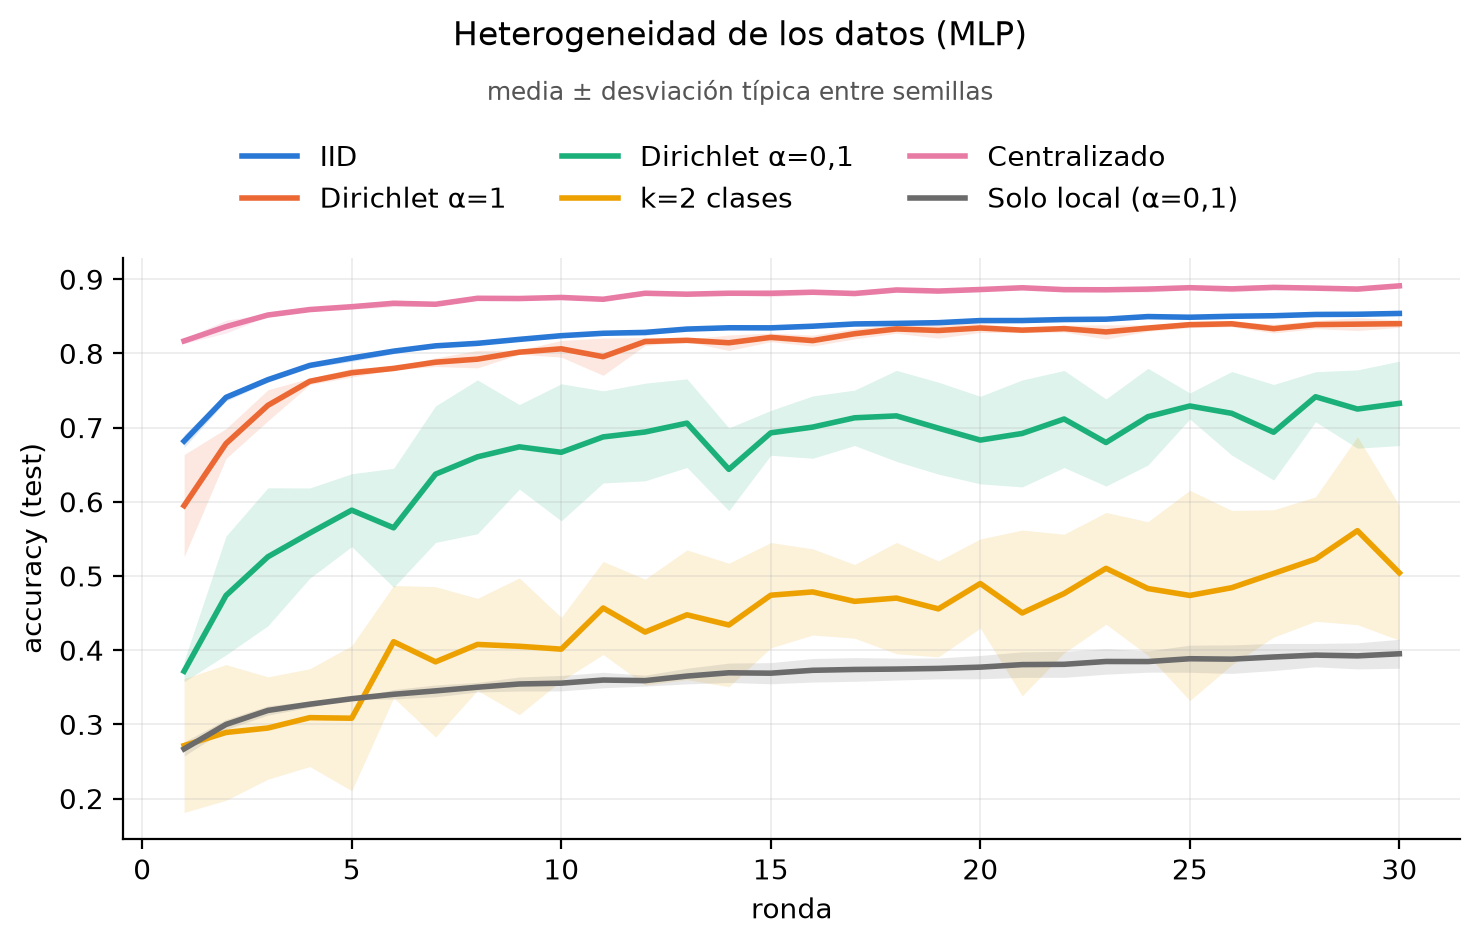
\includegraphics[width=\textwidth]{q1_accuracy.png}
    \caption{\textit{Accuracy} de test por ronda para cada reparto y las dos referencias. La línea es la media
    entre semillas y la banda, $\pm$ una desviación típica.}
    \label{fig:q1_curvas}
\end{figure}

\begin{table}[H]
    \centering
    \caption{Resultados del experimento de heterogeneidad (media $\pm$ desviación típica entre semillas)}
    \label{tab:q1}
    \setlength{\tabcolsep}{5pt}
    \begin{tabular}{lcccc}
        \hline
        Configuración & Semillas & Accuracy final & Oscilación & Salto medio \\
        \hline
        Centralizado & 3 & $0.888 \pm 0.001$ & $0.003 \pm 0.000$ & $0.003 \pm 0.000$ \\
        IID & 5 & $0.852 \pm 0.001$ & $0.003 \pm 0.001$ & $0.002 \pm 0.001$ \\
        Dirichlet $\alpha=1$ & 3 & $0.838 \pm 0.002$ & $0.006 \pm 0.003$ & $0.006 \pm 0.003$ \\
        Dirichlet $\alpha=0.1$ & 5 & $0.722 \pm 0.043$ & $0.034 \pm 0.010$ & $0.040 \pm 0.012$ \\
        Shards $k=2$ & 5 & $0.515 \pm 0.086$ & $0.061 \pm 0.030$ & $0.058 \pm 0.027$ \\
        Solo local & 3 & $0.392 \pm 0.018$ & $0.005 \pm 0.001$ & $0.003 \pm 0.001$ \\
        \hline
    \end{tabular}
\end{table}

\subsubsection{¿Cómo cambia la accuracy final y por qué?}
La \textit{accuracy} final disminuye a medida que aumenta la heterogeneidad de los datos. Básicamente 
porque a medida que la distribución de cada cliente se aleja más de la global, esta métrica empeora.
\\

Con un reparto IID, el valor esperado de la pérdida de cada cliente coincide con la pérdida global,
$\mathbb{E}[F_k(w)] = f(w)$, por lo que todas las actualizaciones locales apuntan aproximadamente hacia el mismo
óptimo y promediarlas se comporta de forma parecida a un SGD centralizado. Con $\alpha=1$ todos los clientes tienen
ejemplos de las 10 clases, aunque en proporciones desiguales, y la pérdida respecto a IID es de solo 1.4 puntos.
\\

Con $\alpha=0.1$ y $k=2$ la caída es mucho mayor (13 y 34 puntos respecto a IID). Cada cliente solo conoce una o
dos clases dominantes, de modo que el óptimo de su función local $F_k$ está lejos del óptimo global. Durante el
entrenamiento local cada modelo se desplaza hacia su propio óptimo (\textit{client drift}) y la media de estos
modelos no coincide con el óptimo de la función global. A esto se suma una convergencia más lenta: entre las
rondas 20 y 30, la curva de $\alpha=0.1$ todavía mejora 4.9 puntos frente a 1 punto en IID. Aun así, según la
teoría, aunque se aumente el número de rondas el resultado se estabiliza por debajo del de IID.
\\

El caso de $k=2$ es el más extremo, ya que la proporción Dirichlet con $\alpha=0.1$ entre las dos clases de cada
cliente hace que, en la práctica, la mayoría tenga una sola clase dominante (Figura~\ref{fig:q1_shards}). 
Además, es la configuración con mayor desviación entre semillas ($\pm 0.086$), porque el reparto depende
de la semilla.
\\

Por último, el solo local obtiene el peor resultado porque cada modelo se evalúa sobre el test global, con las 10
clases equilibradas, pero solo ha visto las pocas clases de su cliente y únicamente es capaz de predecir esas.

\begin{figure}[H]
    \centering
    \begin{minipage}{0.32\textwidth}
        \centering
        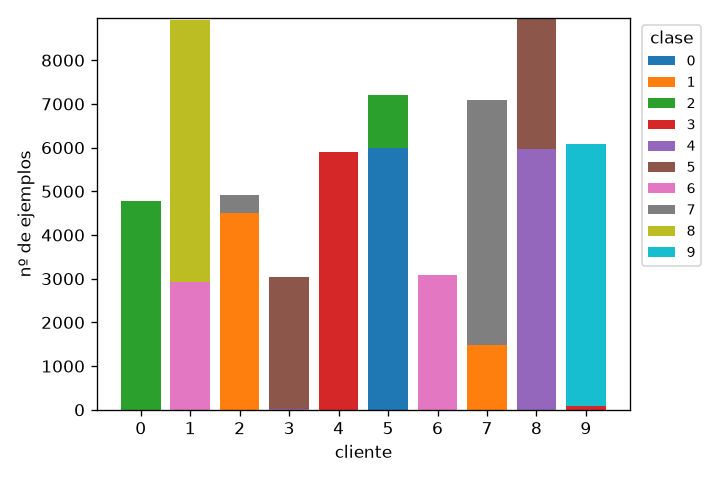
\includegraphics[width=\textwidth]{experiments/1_heterogeneidad/shards_s0.png}\\
        \small Semilla 0 (acc. $0.407$)
    \end{minipage}
    \begin{minipage}{0.32\textwidth}
        \centering
        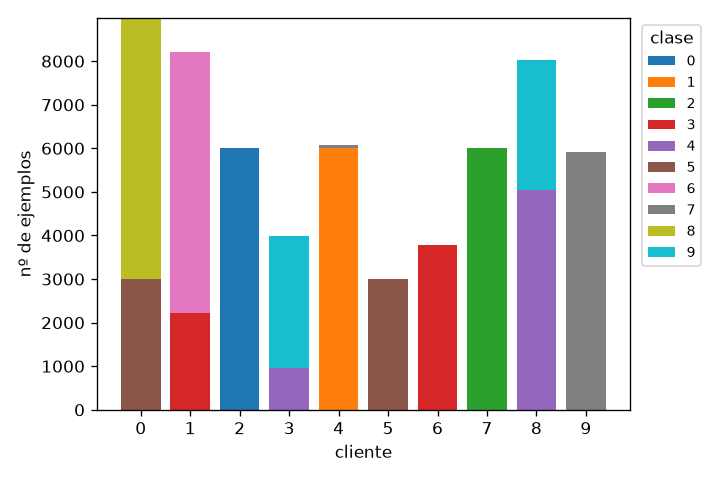
\includegraphics[width=\textwidth]{experiments/1_heterogeneidad/shards_s1.png}\\
        \small Semilla 1 (acc. $0.479$)
    \end{minipage}
    \begin{minipage}{0.32\textwidth}
        \centering
        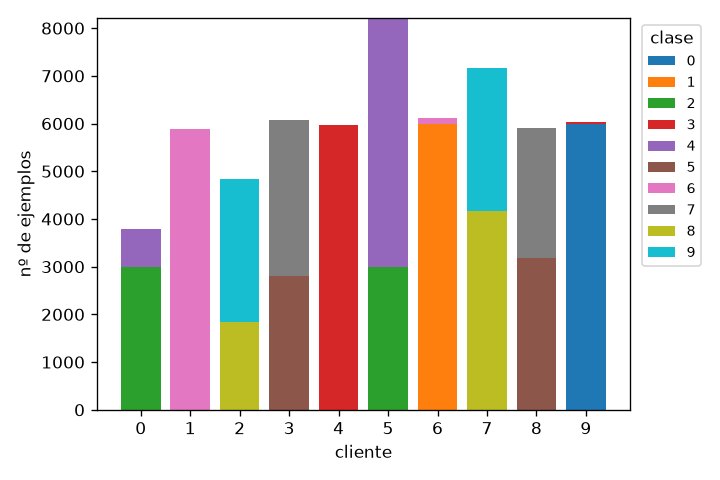
\includegraphics[width=\textwidth]{experiments/1_heterogeneidad/shards_s2.png}\\
        \small Semilla 2 (acc. $0.626$)
    \end{minipage}
    \\[0.3cm]
    \begin{minipage}{0.32\textwidth}
        \centering
        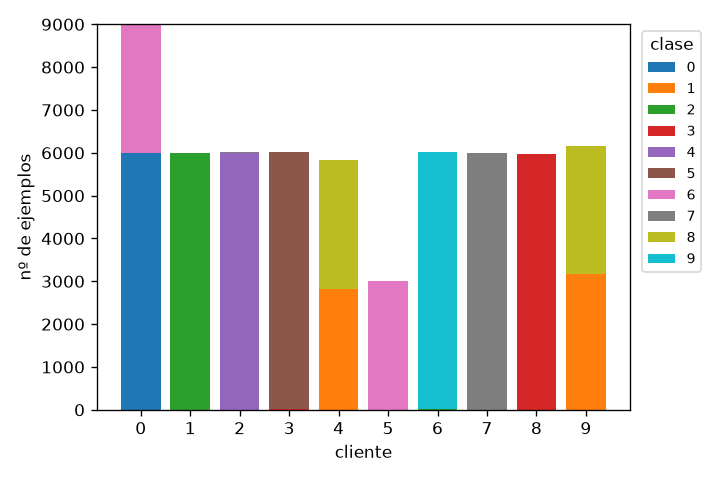
\includegraphics[width=\textwidth]{experiments/1_heterogeneidad/shards_s3.png}\\
        \small Semilla 3 (acc. $0.490$)
    \end{minipage}
    \begin{minipage}{0.32\textwidth}
        \centering
        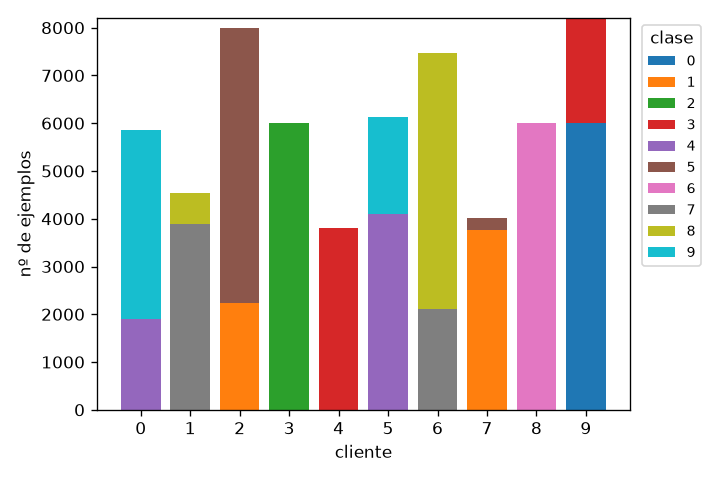
\includegraphics[width=\textwidth]{experiments/1_heterogeneidad/shards_s4.png}\\
        \small Semilla 4 (acc. $0.573$)
    \end{minipage}
    \caption{Reparto Dirichlet Shards ($k=2$, $\alpha=0.1$) con cada semilla y su \textit{accuracy} final.}
    \label{fig:q1_shards}
\end{figure}

\subsubsection{¿Cómo cambia la estabilidad de las curvas y por qué?}
El centralizado, IID y $\alpha=1$ tienen curvas suaves, con una oscilación inferior a $0.006$. Con datos IID
cualquier subconjunto de 5 clientes es representativo de la distribución global, de modo que la actualización
agregada apenas depende de qué clientes se hayan seleccionado en la ronda.
\\

En cambio, la oscilación de $\alpha=0.1$ y $k=2$ es unas 10 y 20 veces mayor que la de IID. Con $C=0.5$ los
clientes seleccionados cambian en cada ronda, y con ellos la mezcla de clases que se entrena: el modelo global se
inclina hacia las clases de los clientes elegidos y empeora en las demás, lo que produce curvas en diente de
sierra.
\\

Por último, el solo local es estable (oscilación de $0.005$) porque no hay muestreo de clientes ni agregación,
pero su curva es prácticamente plana: cada modelo solo sigue ajustando las mismas clases, por lo que en este caso
la estabilidad no indica un buen aprendizaje.

\subsection{Épocas locales}

Experimentos:
\begin{itemize}
    \item $E \in \{1, 5\}$
    \item Particionado: IID y no-IID
\end{itemize}

\subsection{Participación}

\subsection{FedAvg frente FedProx}

\subsection{Comunicación}

\subsection{CNN}

\renewcommand{\refname}{Referencias}
\begin{thebibliography}{4}
\bibitem{mcmahan} McMahan, B., Moore, E., Ramage, D., Hampson, S., Agüera y Arcas, B.: Communication-Efficient
Learning of Deep Networks from Decentralized Data. En: Proceedings of the 20th International Conference on
Artificial Intelligence and Statistics (AISTATS), PMLR 54, pp. 1273--1282 (2017)

\bibitem{hsieh} Hsieh, K., Phanishayee, A., Mutlu, O., Gibbons, P.: The Non-IID Data Quagmire of Decentralized
Machine Learning. En: Proceedings of the 37th International Conference on Machine Learning (ICML), PMLR 119,
pp. 4387--4398 (2020)

\bibitem{groupnorm} Wu, Y., He, K.: Group Normalization. En: Proceedings of the European Conference on Computer
Vision (ECCV), pp. 3--19 (2018)

\bibitem{divergencia} Anónimo: On Federated Learning of Deep Networks from Non-IID Data: Parameter Divergence and
the Effects of Hyperparametric Methods. Envío a ICLR 2020, OpenReview (2019)
\end{thebibliography}



\end{document}